\documentclass[tikz,border=10pt]{standalone}
\begin{document}
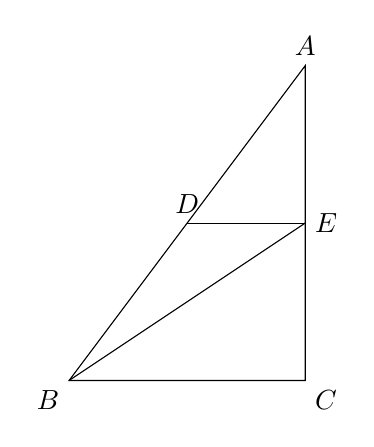
\begin{tikzpicture}
    \coordinate (B) at (0,0);
    \coordinate (C) at (3,0);
    \coordinate (A) at (3,4);
    \coordinate (E) at (3,2);
    \coordinate (D) at (1.5,2);

    \draw (A) -- (B) -- (C) -- cycle;
    \draw (B) -- (E);
    \draw (D) -- (E);

    \node[above] at (A) {$A$};
    \node[below left] at (B) {$B$};
    \node[below right] at (C) {$C$};
    \node[above] at (D) {$D$};
    \node[right] at (E) {$E$};
\end{tikzpicture}
\end{document}
